\subsection{射线和线段}\label{subsec:czjh1-1-2}

我们看图 \ref{fig:czjh1-1-7} , 点 $O$ 是直线 $l$ 上的一个点,它把直线分成两部分。这两部分都是各向一方无限延伸的。
在直线上某一点一旁的部分叫做\zhongdian{射线},这个点叫做\zhongdian{射线的端点}。
探照灯、手电筒的光线都是从一个点向着一个方向射出的,这种光线可以看成射线的具体例子。


\begin{figure}[htbp]
    \centering
    \begin{minipage}[b]{7cm}
        \centering
        \begin{tikzpicture}
	\tkzDefPoints{0/0/O, 1.5/0/x}
	\tkzDrawLine[add=1.0 and 0](O,x)
	\tkzLabelLine[pos=1.0,right](O,x){$l$}
	\tkzDrawPoints[fill=black](O)
	\tkzLabelPoints[above](O)
\end{tikzpicture}


        \caption{}\label{fig:czjh1-1-7}
    \end{minipage}
    \qquad
    \begin{minipage}[b]{7cm}
        \centering
        \begin{tikzpicture}
	\tkzDefPoints{0/0/O, 1.5/0/A}
	\tkzDrawLine[add=0 and 1](O,A)
	\tkzDrawPoints[fill=black](O,A)
	\tkzLabelPoints[below](O,A)
\end{tikzpicture}


        \caption{}\label{fig:czjh1-1-8}
    \end{minipage}
\end{figure}


射线用表示它的端点和射线上任意一点的大写字母来表示,
表示端点的字母写在前面,如射线 $OA$ (图\ref{fig:czjh1-1-8})。

如果点 $A$、$B$ 是直线 $l$ 上的两个点,这两个点将直线 $l$ 分成了三部分(图\ref{fig:czjh1-1-9})。
直线上两点间的部分叫做\zhongdian{线段},这两点叫做\zhongdian{线段的端点}。
图\ref{fig:czjh1-1-9} 中的第 II 部分就是以点 $A$、$B$ 为端点的线段。
书桌的一条棱、直尺的一边都给我们以线段的形象。

\begin{figure}[htbp]
    \centering
    \begin{minipage}[b]{6cm}
        \centering
        \begin{tikzpicture}
	\tkzDefPoints{0/0/A, 1.5/0/B}
	\tkzDrawLine[add=1.0 and 0.8](A,B)
	\tkzLabelLine[pos=1.8,right](A,B){$l$}
	\tkzLabelLine[pos=-0.5,above=.5em](A,B){I}
	\tkzLabelLine[pos=0.5, above=.5em](A,B){II}
	\tkzLabelLine[pos=1.4, above=.5em](A,B){III}
	\tkzDrawPoints[fill=black](A,B)
	\tkzLabelPoints[above](A,B)
\end{tikzpicture}


        \caption{}\label{fig:czjh1-1-9}
    \end{minipage}
    \qquad
    \begin{minipage}[b]{9cm}
        \centering
        \begin{minipage}[b]{3cm}
            \centering
            \begin{tikzpicture}
	\tkzDefPoints{0/0/A, 1.5/0/B}
	\tkzDrawSegment(A,B)
	\tkzDrawPoints[fill=black](A,B)
	\tkzLabelPoints[above](A,B)
\end{tikzpicture}


            \caption*{甲}
        \end{minipage}
        \quad
        \begin{minipage}[b]{3cm}
            \centering
            \begin{tikzpicture}
	\tkzDefPoints{0/0/A, 1.5/0/B}
	\tkzDrawSegment(A,B)
	\tkzLabelSegment[above](A,B){$a$}
	\tkzDrawPoints[fill=black](A,B)
\end{tikzpicture}


            \caption*{乙}
        \end{minipage}
        \caption{}\label{fig:czjh1-1-10}
    \end{minipage}
\end{figure}


线段用表示它的两个端点的两个大写字母来表示,也可以用一个小写字母来表示。
如图 \ref{fig:czjh1-1-10} 甲中的线段记作线段 $AB$ 或线段 $BA$,
图 \ref{fig:czjh1-1-10} 乙中的线段记作线段 $a$。

如图 \ref{fig:czjh1-1-11}, 线段 $AB$ 可以向任意一方延伸。线段向一方延伸的部分叫做\zhongdian{线段的延长线}。
对于图 \ref{fig:czjh1-1-11} 甲常说成 “延长线段$AB$”;
对于图 \ref{fig:czjh1-1-11} 乙常说成 “延长线段$BA$”,有时也说成 “反向延长线段$AB$”。

\begin{figure}[htbp]
    \centering
    \begin{minipage}[b]{6cm}
        \centering
        \begin{tikzpicture}
	\tkzDefPoints{0/0/A, 1.5/0/B, 3/0/x}
	\tkzDrawSegment(A,B)
	\tkzDrawSegment[dashed](B,x)
	\tkzDrawPoints[fill=black](A,B)
	\tkzLabelPoints[above](A,B)
\end{tikzpicture}


        \caption*{甲}
    \end{minipage}
    \qquad
    \begin{minipage}[b]{6cm}
        \centering
        \begin{tikzpicture}
	\tkzDefPoints{0/0/A, 1.5/0/B, -1.5/0/x}
	\tkzDrawSegment(A,B)
	\tkzDrawSegment[dashed](A,x)
	\tkzDrawPoints[fill=black](A,B)
	\tkzLabelPoints[above](A,B)
\end{tikzpicture}


        \caption*{乙}
    \end{minipage}
    \caption{}\label{fig:czjh1-1-11}
\end{figure}

在这一节里,我们讲了射线、射线的端点、线段、线段的端点、线段的延长线等名词,对于一个名词我们需要说明它的含意。
例如,用 “直线上两点间的部分” 来说明 “线段” 的含意,这样的语句叫做\zhongdian{名词的定义}。


\begin{lianxi}

\xiaoti{口答:}
\begin{xiaoxiaotis}

    \xxt{怎样表示图甲中以 $O$ 为端点的各条射线?}

    \xxt{怎样表示图乙中以 $O$ 为端点的各条射线?}

    \xxt{图乙中射线 $DE$ 和射线 $OE$ 是同一条射线吗?图乙中射线 $DE$ 与射线 $ED$; 射线 $DO$ 与射线 $DE$ 呢?}

\end{xiaoxiaotis}

\begin{figure}[htbp]
    \centering
    \begin{minipage}[b]{6cm}
        \centering
        \begin{tikzpicture}
	\tkzDefPoints{0/0/O, 1.5/0.7/A, 1.5/0/B, 1.5/-0.7/C}
	\tkzDrawLines[add=0 and 0.5](O,A  O,B  O,C)
	\tkzDrawPoints[fill=black](O,A,B,C)
	\tkzLabelPoints[left](O)
	\tkzLabelPoints[above](A,B,C)
\end{tikzpicture}


        \caption*{甲}
    \end{minipage}
    \qquad
    \begin{minipage}[b]{6cm}
        \centering
        \begin{tikzpicture}
	\tkzDefPoints{0/0/D, 1/0/O, 2/0/E}
	\tkzDrawLines[add=0.2 and 0.2](D,E)
	\tkzDrawPoints[fill=black](D,O,E)
	\tkzLabelPoints[above](D,O,E)
\end{tikzpicture}


        \caption*{乙}
    \end{minipage}
    \caption*{(第 1 题)}
\end{figure}


\xiaoti{图甲、乙中各有几条线段?用字母表示各条线段。}


\begin{figure}[htbp]
    \centering
    \begin{minipage}[b]{9cm}
        \centering
        \begin{minipage}[b]{3cm}
            \centering
            \begin{tikzpicture}
	\tkzDefPoints{0/0/A, 2/0/B, 1.3/0.9/C}
	\tkzDrawPolygon(A,B,C)
	\tkzLabelPoints[above](C)
	\tkzLabelPoints[below](A,B)
\end{tikzpicture}


            \caption*{甲}
        \end{minipage}
        \qquad
        \begin{minipage}[b]{5cm}
            \centering
            \begin{tikzpicture}
	\tkzDefPoints{0/0/D, 1/0/E, 1.7/0/F, 2.6/0/G}
	\tkzDrawSegment(D,G)
	\tkzDrawPoints[fill=black](D,E,F,G)
	\tkzLabelPoints[below](D,E,F,G)
\end{tikzpicture}


            \caption*{乙}
        \end{minipage}
        \caption*{(第 2 题)}
    \end{minipage}
    \qquad
    \begin{minipage}[b]{6cm}
        \centering
        \begin{tikzpicture}
	\tkzDefPoints{0/0/A, 2/1/B, 2/0/C, 0.3/1.3/D}
	\tkzDrawPoints[fill=black](A,B,C,D)
	\tkzLabelPoints[above](D)
	\tkzLabelPoints[right](B,C)
	\tkzLabelPoints[below](A)
\end{tikzpicture}


        \caption*{(第 4 题)}
    \end{minipage}
\end{figure}

\xiaoti{射线、线段各有几个端点? 直线有没有端点?}

\xiaoti{如图,已知四点 $A$、$B$、$C$、$D$。读下列语句,并画出图形。}
\begin{xiaoxiaotis}

    \xxt{“连结 $AB$” (即画出以点 $A$ 和点 $B$ 为端点的线段),并延长线段 $AB$;}

    \xxt{“连结 $CD$”,并延长线段 $DC$, 线段 $AB$、$CD$ 交于点 $O$;}

    \xxt{“连结 $BC$”,并反向延长线段 $BC$。}

\end{xiaoxiaotis}


\xiaoti{说出线段的延长线的定义。}

\end{lianxi}

